%SourceDoc ../YourName-Dissertation.tex
\chapter{Introduction -- Urban Computing} \label{chapter1:introduction}



With the advent of information age, more and more data are collected in the urban space. Using various urban data to solve real urban problem is called urban computing.



\section{The Challenges and Opportunities from Urban Data}


Urban data have the following three main properties. 

\textbf{Variety} refers to the heterogeneous data sources. As shown in Figure~\ref{fig:demo-data}, there is various types of data in the urban space. In the city, we can collect traffic data, Point-of-interest (POI), air quality measure, weather,  city noise complaints, and many more. Different types of data lead to different format in the data. For example, the air quality measure and weather is global over the city. Meanwhile, the crime incidents and taxi trip data have specific location information.


\textbf{Volume} of urban data is generally large. For example, there are more than $380,000$ POIs in New York City and $112,000$ POIs in Chicago. According to the Chicago public crime incidents record, there are over $5.8$ millions of records in the past 15 years. Each of the crime records have detailed information on the date, location, and crime description. 


\textbf{Velocity} refers to the speed that new data is generated, which is also huge in the urban space. For example, there are almost half million taxi trips are generated in New York City each day, and there are 621 millions of tweets posted each day.


All the large volume and heterogeneity of urban data poses a challenge for us to study. At the same time, those data enables the opportunities to look into many urban problems, such as traffic anomaly detection,  travel time estimation, city noise diagnosing, from a new angle.


\begin{figure}[h]
\centering
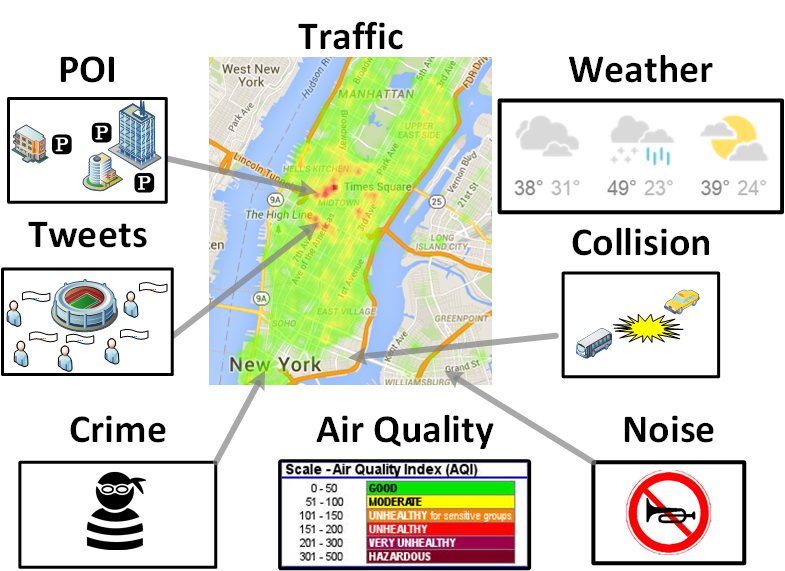
\includegraphics[width=0.9\textwidth]{fig/intro-data.png}
\caption{Use data collected in the urban space to address real urban problems.}
\label{fig:demo-data}
\end{figure}



\subsection{A New Type of Data: Mobility Flow}


As the advance to positioning technology, we are able to collect more and more mobility data.
In the urban space, the trajectories of massive public transportation vehicle are recorded at minute intervals; the taxi/urban trips are recorded by pickup/drop-off locations and time; personal trajectories are tracked by health related mobile App, people's home and office location are surveyed by US Census Bureau.


The mobility data is a new type of data, because it is not attached to one specific point as most of other urban data.
The mobility data tracks the movement of people among two or several locations. The ability to connect various locations make the mobility data unique and important~\cite{ZCWY14}.




\section{Model Interactions In Urban Space}



\subsection{Traditional Approach: Space Continuity}


City is a huge and complicated system, where everything might be connected. Building a new transportation center may incur more traffic as well as crime incidents in the nearby areas. When a big event happens and a lot of people accumulate at the venue, the traffic volumes at nearby regions increase as well. From the example above, we see that various interactions are undergoing among different regions in the city.


In the traditional urban computing research literature, the most widely used and accepted assumption is \textbf{space contiguity}, which assumes that spatially adjacent regions tend to have similar properties. In urban space, most data reflect the properties of human beings, such as the traffic volume, crime count, and geo-tagged tweets. Therefore, these data are attached to human crowd instead of a specific location. 
In the urban space, the intuition behind the \textbf{space continuity} is that human movement is regular, and most of our daily activities are conducted in a limited area. Based on the space continuity assumption, when studying the interactions among regions, it is naturally to assume that geographically adjacent regions tend to be more alike.  Examples are high-crime community tend to have bad influence on its neighboring community, and vice versa.



\subsection{New Approach: Flow as Hyperlink}

When the human mobility data is not widely available, the space continuity makes a lot of sense. However, the new mobility flow data enables us to build better model of \textbf{region interactions} with the real human movement.
\emph{In my proposal, my research focus is to capture the complicated interactions in the urban space with the new flow data}.



\textbf{Take crime inference as an example}. Understanding how to control crime is important because exposures to violence and crime have been unusually high in the U.S. for several decades and, while declining, they remain high~\cite{Baum05, Fink08}.Over half a million children and youth aged 10-24 years were treated in 2012 in emergency departments for nonfatal physical assault injuries related to gun shots, cuts and stabbings, among others~\cite{cdc15}.  Understanding the neighborhood context of crime is particularly important because victimization and other forms of crime exposures have many severe consequences.  Beyond the high medical bills and violent death, consequences include behavioral and mental health problems, aggression, substance abuse, post-traumatic stress disorder, and suicide, lower academic achievement, and engaging in further violence~\cite{Grai15}. 


\begin{figure}[t]
\centering
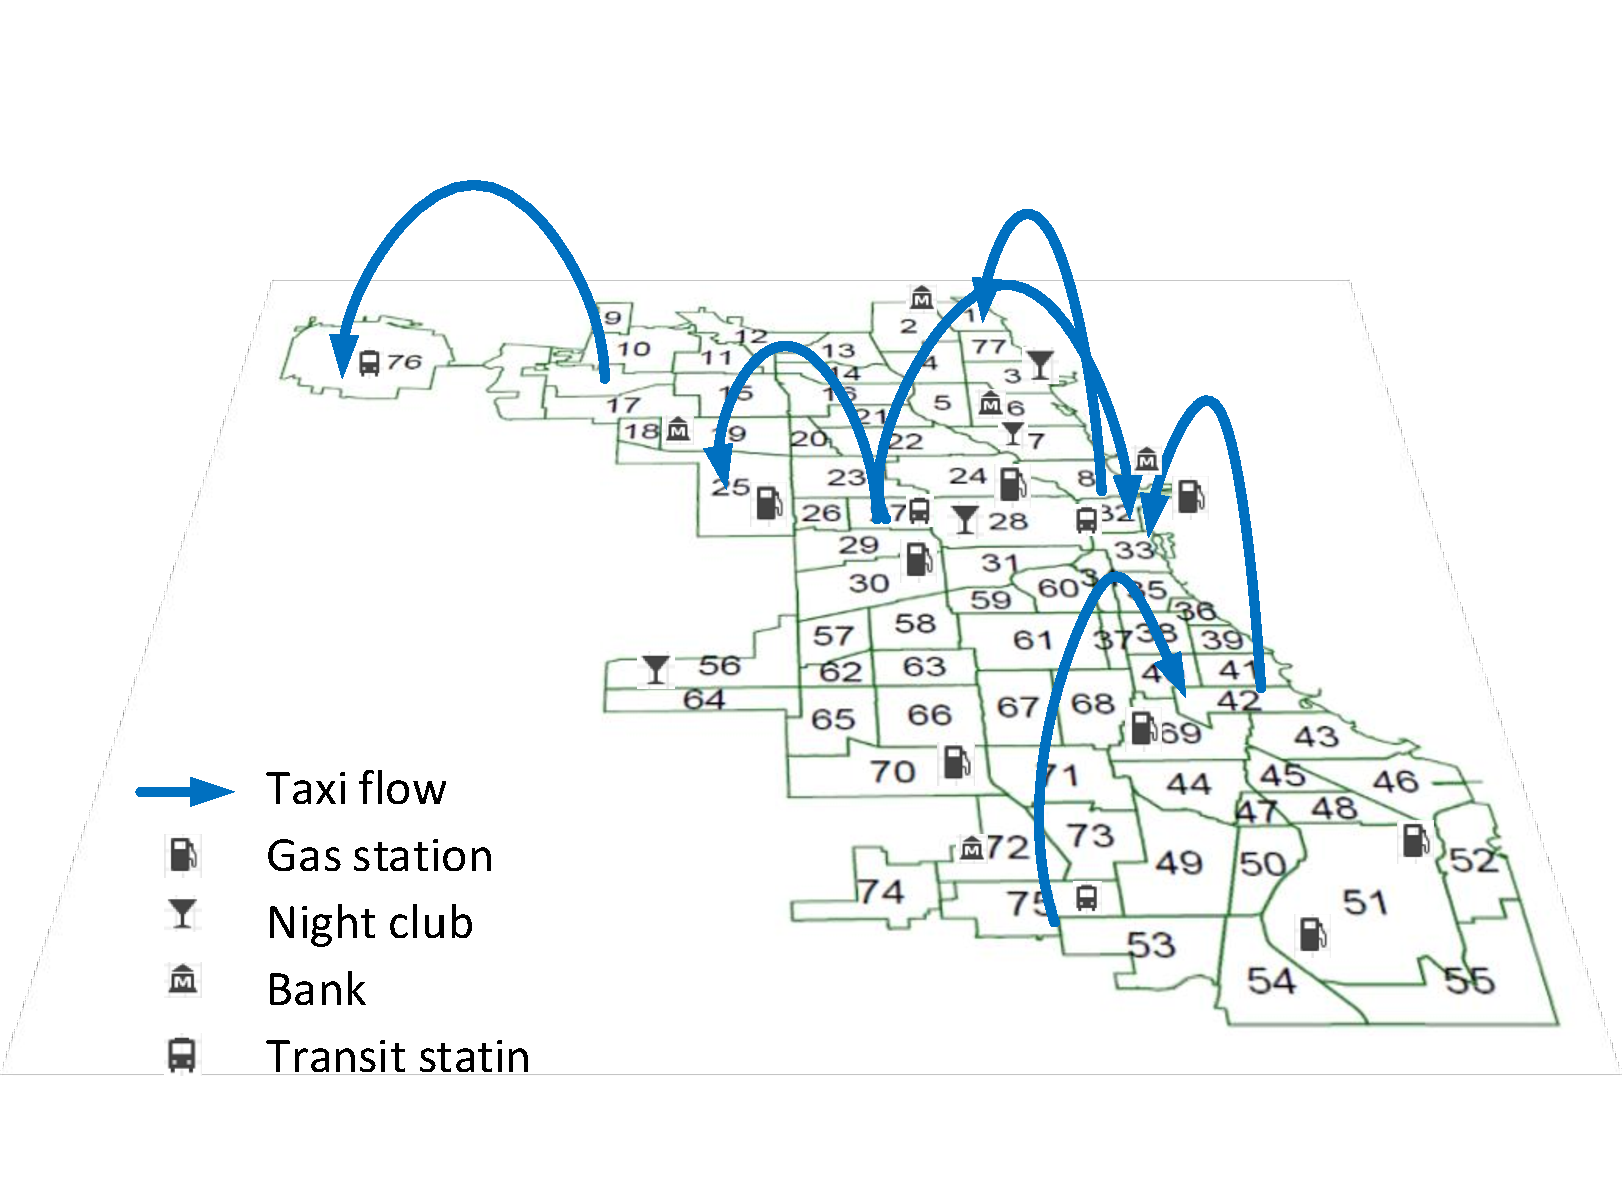
\includegraphics[width=0.8\textwidth]{fig/demo.pdf}
\caption{An illustration of various types of features we used in Chicago. The POI distribution across community areas reflects profiles of the region functionality. The taxi flow connects nonadjacent regions and act as a ``hyperlink''.}
\label{fig:demo}
\end{figure}

Traditionally, researchers have used demographic information (e.g., population poverty level, socioeconomic disadvantage, racial composition of population) to estimate the crime rate in a community~\cite{GrSa09}. However,  such demographic information only contains partial information about the neighborhoods and does not dynamically reflect the changes in the community (demographic survey is conducted by census bureau every 10 years). Using only demographic information will result in a relative error of at least 30\% for crime rate estimation in Chicago (refer to experiment section in the paper). Existing studies also use the geographical influence~\cite{Ans02} to estimate the crime rate, i.e., the crime in the nearby communities can be propagated to the focal community. But this geographical influence is of little help in improving the crime inference on top of demographic feature, with at most 0.4\% relative improvement in our experiments. This is probably because the nearby communities also share similar demographics, which limits the additional benefit of geographical influence.



In Figure~\ref{fig:demo}, we show that taxi flow as a newer type of big data could provide us new insights to understand some traditional socioeconomic urban problems.  A huge amount of taxi flow data reflect how people commute in the city. In previous studies, when using geographical influence~\cite{Ans02}, people assume that a community is affected by the spatially nearby communities. However, communities are not only affected by spatially-close communities. Even if two communities are distant in geographical space, they could have a strong correlation if there are many people frequently travel between these two communities~\cite{GGM14}. We hypothesize that taxi flows may be considered as ``hyperlinks'' in the city that connect the locations and we use such data to estimate crime rates. Our experiments show very promising results --  adding taxi flow data on top of all other features can further decrease the error by 5\%.










\section{Proposed Research Questions}



In the urban space, \textbf{region interactions} bring solutions to the following several fundamental data mining questions. We propose to view the city as a spaital network of communites linked by ``hyperlink'' flow.
\begin{itemize}
\item Understand nodes using links. Estimate an unobserved property of focal community, given the observations on other communities and other types of data. For example, the crime rate in a residential neigborhood could be impacted by  non-adjacent but flow-connected neighborhoods, because the residents in the neighborhoods are also exposed to and influenced by the environment in the workplace.
\item Understand links using nodes. Are certain properites of two connected nodes associated with the type and volume of the flow connections? For example, given the crime profiles of two connected communities, which type of interactions (taxi, LEHD, or space continuity) is more important in forming the crime properties?
\item Identify the fundamental dependency structure among properties of nodes. For example, the crime rate of two connected communities may show a strong correlation. However, this does not necessarily mean that high crime rate in one community lead to the high crime in another. The crime is very likely to be caused by other properties. 
\end{itemize}